% File: css-ot.tex

\documentclass{standalone}

\usepackage{tikz}
\usetikzlibrary{shapes, positioning, arrows.meta, calc, intersections, backgrounds, fit}

% default horizontal/vertical distance
\def\hdist{1.5}
\def\vdist{1.5}

\newcommand{\state}[3]{% #1: state name; #2: position; #3: state label
  \node (#1) [circle, inner sep = 0pt, minimum size = 10mm, text width = 10mm, align = center, draw, #2, font = \Large] {#3};
}

\newcommand{\trans}[5]{% #1: start state; #2: end state; #3: transition label; #4: transition label position; #5: style
  \draw[>=Stealth, ->,  #5] (#1) to node [rectangle, draw, above = 2pt, sloped, #4] {#3} (#2);
}

\newcommand{\transition}[4][]{% #2: start state; #3: end state; #4: transition label; #1: transition label position (optional)
  \draw[>=Stealth, ->] (#2) to node [rectangle, draw, above = 2pt, sloped, #1] {#4} (#3);
}

\tikzset{node distance = \vdist and \hdist}
\tikzset{path/.style = {draw, rounded corners, very thick, #1}}

\begin{document}
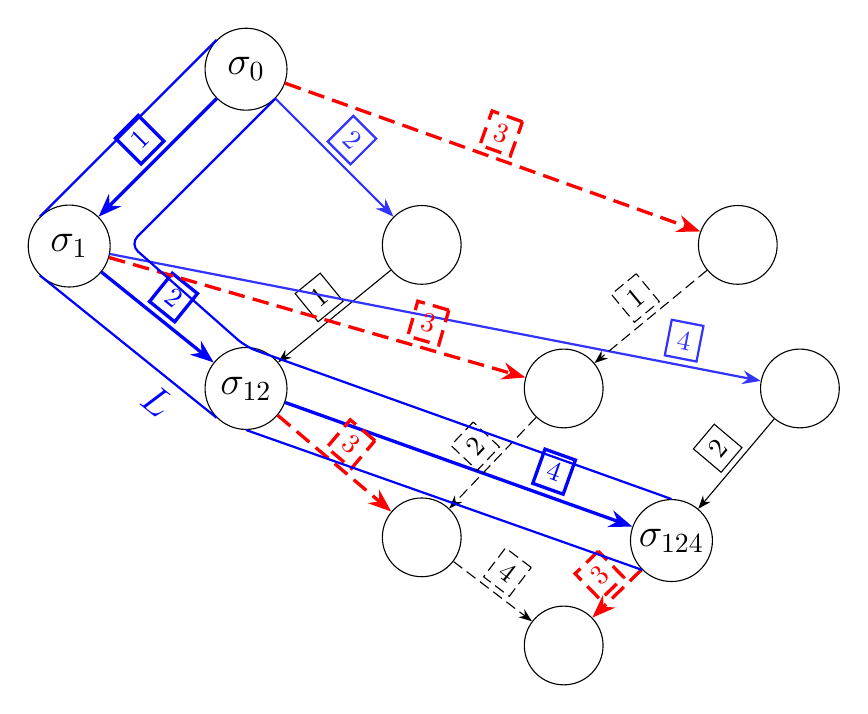
\begin{tikzpicture}[
	add/.style = {dash pattern = on 4pt off 2pt},
	lstyle/.style = {blue, very thick},
	ostyle/.style = {red, very thick, dash pattern = on 6pt off 3pt},
	atrans/.style = {thick, blue!80}]
  \state{0}{}{$\sigma_{0}$}
  \state{1}{below left = of 0}{$\sigma_{1}$}
  \state{2}{below right = of 0}{}
  \state{12}{below = 2*\vdist of 0}{$\sigma_{12}$}
  \trans{0}{1}{1}{}{lstyle}
  \trans{0}{2}{2}{}{atrans}
  \trans{1}{12}{2}{}{lstyle}
  \trans{2}{12}{1}{}{}

  \state{3}{right = 2*\hdist of 2}{}
  \trans{0}{3}{3}{}{ostyle}
  \state{14}{right = 4*\hdist of 12}{}
  \state{124}{below left = 0.80*\vdist and 0.6*\hdist of 14}{$\sigma_{124}$}

  \trans{1}{14}{4}{very near end}{atrans}
  \trans{12}{124}{4}{near end}{lstyle}
  \transition{14}{124}{2}

  \state{13}{right = 2*\hdist of 12}{}
  \trans{1}{13}{3}{near end}{ostyle}
  \trans{3}{13}{1}{}{add}

  \state{123}{below = 1.8*\vdist of 2}{}
  \trans{12}{123}{3}{}{ostyle}
  \trans{13}{123}{2}{}{add}

  \state{1234}{below = 1.5*\vdist of 13}{}
  \trans{123}{1234}{4}{}{add}
  \trans{124}{1234}{3}{}{ostyle}

  \path [name path = 12-1] (12.north) -- (1.north east);
  \path [name path = 1-0] (1.south east) -- (0.south east);
  \path [name intersections = {of = 12-1 and 1-0, by = x}];
  % \node [red, circle] at (x) {x};

  \draw[rounded corners, blue, thick] (0.north west) -- (1.north west) 
	(1.south west) to node[near end, below, sloped, blue, font = \Large] {$L$} (12.south west)
	(12.south) -- (124.south west)
	(124.north) -- (12.north) -- 
	(x) -- (0.south east);
\end{tikzpicture}
\end{document}
